\chapter{Deep Learning and Curriculum Learning}
Humans are different from other species in many ways, but two of them are particularly noteworthy. 
First of all, humans display an exceptional capacity to learn;
moreover, humans are remarkable for the long time they take to reach maturity. Human beings need about two decades to be trained as fully functional adults for our society and it may
be argued that, through culture, learning has created the basis for a non-genetically based transmission of behaviors and habits which might
accelerate the evolution of our species. Infancy and childhood are times of great vulnerability for the young, when the first skills are developed and when the adults who
must care for and protect their own young go through a severe restriction of their range of activities. Then, why would evolutionary process not prune a long period of 
immaturity from our species? Previous research carried out by Elman \textit{et al} \cite{ELMAN199371} at the intersection of cognitive science
and machine learning underline that it is important to remember that the evolution looks at the whole individuals rather than at the value of isolated traits; the adaptive success of individuals therefore is 
determined by the joint interaction of all their traits. Thus, it might be that to understand the persistence of one trait with apparently negative consequences - such as the lenghty period of immaturity, possible interactions
with other traits - such as the ability to learn - may need to be considered. The perfect example of such an interaction, is that in human beings the greatest learning occurs precisely in the period of time
when they are undergoing major changes, during childhood indeed.\\

\section{State of the art}
In humans, learning and development interact in a way as important as non-obvious; maturational changes might provide the enabling 
conditions which allow learning to be most effective. It is a matter of fact that humans need about two decades to be trained as fully functional 
adults, and the higher the training is organized, the better the knowledge of the person. Humans in fact learn much better when the examples are not randomly presented, but organized in such a way 
where the amount of concepts is incremented gradually, and where the complexity of them increases over time. The majority of education systems are organized in order to illustrate 
different concepts at different times, exploiting previously learned notions to ease the learning of new abstractions. By choosing which examples to present and in which order to explain them to the learning system, one can guide
training and consequently increase the speed at which learning can happen. This is the same idea exploited in \textit{animal training} by psychologists Skinner (1958), Peterson (2004) and Krueger \& Dayan (2009)
where it is called \textit{shaping}. \\
In the context of machine learning, such a meaningful learning process is known as \textit{curriculum learning}, whose basic idea - traced back to Elman - is to start small, learn easier aspects
of the task, and then gradually increase the difficulty level.
Inspired by human learning in fact, curriculum learning (CL) is a training strategy that emphasizes
the order of training instances in a computational learning setup.
As a feature of human learning, curriculum - or even better learning in a meaningful way -
has been transferred to machine learning, thus creating the subdiscipline named
\textit{curriculum learning}.
Essentially, human education is organized as curricula, by starting small indeed, and gradually presenting more complex
concepts. The paramount hypothesis is that simpler instances should be learned
during the first steps as building blocks, to then learn more complex ones. Several experiments on sentiment 
analysis task and tasks similar to sequence prediction tasks in NLP carried on by Cirick \textit{et al} \cite{Cirik2016VisualizingAU} prove that
curriculum learning has positive effects on LSTM's internal states, by biasing the model through building constructive representations. 
Specifically, the internal representation at the previous timestep is used as building block for the next one, thus
contributing at the final prediction.

In traditional machine learning algorithms all the training examples are randomly presented to the model,
thus ignoring the different complexities of data instances and the learning status of the current model. 
Owning to this, it is fairily intuitive wondering if the curriculum training strategy could ever benefit machine learning.
Extensive experiments from early \cite{bengio2009curriculum}, \cite{kumar2010self}, \cite{zaremba2014learning} to recent works \cite{fan2018learning}, \cite{graves2017automated}, \cite{hacohen2019power}, \cite{platanios2019competence} in various applications of machine learning show that such strategy is of benefit to this field, but not always, and 
because of that the power of introducing the curriculum-like strategy depends on how the curriculum for specific applications and datasets is designed.

\section{Curriculum Learning related works}
As the idea of CL provide a general training strategy beyond specific machine learning
tasks, its power have been exploited in considerably wide application scopes, including supervised learning
tasks within computer vision, natural language processing (NLP), healthcare prediction, various
reinforcement learning (RL) tasks, as well as other applications such
as graph learning, and neural architecture search (NAS). As already mentioned in \ref{chapter:MAO}, the advantages of applying CL
training strategies to miscellaneous real-world scenarios can be mainly summarized as (i) improving the model perfomrance on 
target tasks, and (ii) accelerating the training process, which cover the two most significant 
requirements in most of the machine learning research. 
To provide an illustration,
Platanios \textit{et al.} \cite{platanios2019competence} present 
a personal framework that consists of a way of deciding which training instances
are shown to the model ad different times during training, based on 
an estimated difficulty of a sample and on the current competence
of the model. Thus, filtering training samples prevents the model from 
getting stuck in bad local optima, making it converge faster and reach
a better solution than the common approach of uniformly 
sampling training examples. Their experiment shows that CL helps the 
neural machine translation model reduce training time by up to 70\%, whie at the 
same time obtaining accuracy improvements of up to 2.2 BLEU points, compared
to plain training without any curricula. In \cite{florensa2017reverse} Florensa 
\textit{et al.} talk about curriculum learning as a reverse curriculum technique. 
They propose a method to learn goal-oriented tasks without requiring
any prior knowledge, other than obtaining a single state in which
the task is achieved. They dimonstrate that their approach is 
based on a reverse training, where the robot gradually learns to reach 
the goal from a set of start states increasingly far from the goal.
That approach resulted in solving hard problems, not solvable 
by state-of-the-art reinforcement learning methods.

\section{Curriculum Learning application in Deep Learning tasks}
Training neural networks is traditionally done by providing a sequence of 
random mini-batches sampled uniformly from the entire training data. Conversely, curriculum learning
involves the non-uniform sampling of mini batches, on the training of deep networks.
However, understanding why and when \textit{starting small} strategies can 
benefit machine learning algorithms is a question that every scholar try to contribute to.
Bengio \textit{et al.} \cite{bengio2009curriculum} other than showing several cases where very simple
multi-stage curriculum strategies give rise to improved generalization and faster convergence, 
contribute to the question introducing a hypothesis which might help to explain 
some of the advantages of a curriculum strategy. They argue that a well chosen curriculum 
strategy can act as a continuation method. Intuitively, continuation methods are optimization
strategies for non-convex criteria which first optimize a smoother and easier version of the problem to 
reveal the "global picture", and then gradually consider less smoothing versions, until the tarhet objective of 
interest. Therefore, continuation methods provide a sequence of optimization objectives, starting with an objective for which
it is easy to find a global minimum, and tracking the local minima throughout the training. In this way, continuation methods
guide the training towards better regions  and the local minima learned from easier objectives have better
generalization ability and are more likely to approximate global minima.
To test this hypothesis, they turn the attention to training of deep
architectures, which have been shown to involve good solutions in local minima that are almost impossible to find 
by \textit{random initialization}. Generally, deep learning methods try 
to learn feature hierarchies, i.e., features at higher levels are formed by the composition of lower level features.
As a consequence, automatically learning multiple levels of abstracion may allow a system to induce complex functions mapping the input to the 
output directly from data, without depending heavily on human-crafted features.
One possible theoretical motivation for deep architectures comes from complexity theory. Some functions, in fact, can 
be represented with an architecture of depth \textit{k} but require an exponential size architecture when the depth 
is restricted to be less than \textit{k}. Training deep networks, however, involves a potentially 
intractable non-convex optimization problem \cite{bengio2009curriculum}. There were no good algorithms for training 
fully-connected deep architectures before 2006, when Hinton introduced a learning algorithm that greedily trains one layer at a time, exploiting an unsupervised
generative learning algorithm for each layer. It is conceivable that by training 
each layer one after the other, the network is organized in such a way that it can first learn the simpler
concepts, represented in the first layer indeed, then sligthly more abstract ones, represented in the second layer, and so on.
Not long after, strategies for building deep architectures from related variants were proposed %add ref 
and these works showed the advantage of those frameworks over shallow ones, and of the unsupervised 
pre-training strategy in a variety of settings.\\

\section{Definition of Curriculum Learning}
Based on all the previous works in the first place provided in behavior and 
cognitive science literature, the concept of CL was first proposed in \cite{bengio2009curriculum} with 
experiments on supervised visual and language learning tasks, exploring when and why curriculum could benefit machine learning.
The original definition of CL refers to a curriculum as a sequence of training criteria 
over \(T\) training steps \( C = \left \langle Q_1, ..., Q_t, ..., Q_T \right \rangle\), where each  
criterion \(Q_t\) is a reweighting of the target training distribution \(P(z)\): \(Q_t(z) \propto W_t(z)P(z)\), for 
each instance in the training set. In the definition the following three conditions were considered:
\begin{itemize}
    \item the entropy of distributions gradually increases, \(H(Q_t) < H(Q_{t+1})\);
    \item the weight for any example increases, \(W_t(z) \leq W_{t+1}(z) \forall z \in D\);
    \item \(Q_T(z) = P(z)\).
\end{itemize}
So, curriculum learning is the training strategy that trains a machine learning model
with a curriculum. The first of the above conditions means that the diversity 
and the information of the training set should gradually increase. More specifically,
the reweighting of examples in later steps increases the probability of sampling slightly more difficult examples.
The second condition instead means to gradually add more training examples, letting the size of the training set increase. 
Finally, the last condition
means that the reweighting of all examples is uniform and the training is carried on the target training set.\\
At a more abstract level, a curriculum can be seen as a sequence of instance selection or example reweighting along the training process in order to achieve faster convergence or better generalization, 
which is beyond the "easy to hard" or "starting small" principles. 

\section{A general CL framework}
In a nutshell, curriculum learning means "training from easier data to harder data" \cite{Wang2020}. More specifically the
core idea is to "start small" \cite{ELMAN199371}, train the machine learning model with easier subtasks, to then gradually increase
the difficulty level of subtasks until the whole training dataset is used.\\
Bearing in mind the strategy of training from easier to harder data, to design such a curriculum idea 
(i), what kind of training data is supposed to be easier than other data, (ii) and when is appropriate to present more harder
data for training - and how much more - must necessarily be decided.
Technically, those 2 issues can be abstracted in the concepts of a Difficulty Measurer, that decides the "easiness"
of each data instance to start the training process from, and a Training Scheduler, that rules the sequence of data subsets during 
the whole training process \cite{Wang2020}.
Therefore, Difficulty Measurer together with Training Scheduler constitute a general framework for curriculum design,
as illustrated in Figure ~\ref{fig:CLdesign}.
\begin{figure}[h]
    \begin{center}
        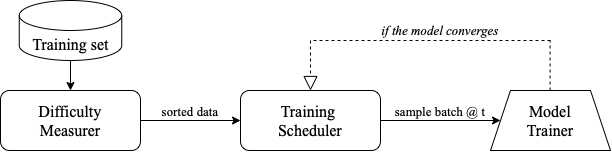
\includegraphics[width=0.55\textwidth]{/Users/carmenarmenti/Desktop/Thesis document/images/predefinedCL.png}
        \caption{\label{fig:CLdesign}Predefined Curriculum Design.}
    \end{center}
\end{figure}
First of all, the Difficulty Measurer sorts all the training examples from the easiest 
to the hardest and passes them to the Training Scheduler. Then, at each training epoch \textit{t}, the Training Scheduler
samples a batch of training instances from the easier subset and gives them to the Model Trainer for training.\\
As training epochs increase, the Scheduler decide when to sample from more harder data, generally until uniform sampling
from the whole training set. This schedule either depends on the training loss feedback from the Model Trainer, or on some other
parameters that implies that the model would deverge, if left to training for more epochs.\\
Moreover, a distinction between \textbf{predefined CL} and \textbf{automatic CL} must be clarified. The first refers to the framework
where both the Difficulty Measurer and Training Scheduler are defined by human prior knowledge, thus with no data-driven
algorithms involved; the latter instead, if any - or both - of the components are designed by data-driven algorithms.\\
Usually, the power of introducting Curriculum into Machine Learning depends on how the curriculum for specific
applications and dataset is designed. Due to this, Difficulty Measurers often relies on the data
characteristics of specific tasks, and most of them are defined by complexity, diversity, or noise estimation
definitions.\\

%%%%%%%%%%%%%%%%%%%%
% NOTES
% As mentioned previously, this is the first work studying LSTM networks
% on software engineering tasks with curriculum learning to our knowledge.

%%%%%%%%%%%%%%%%%%%%